\documentclass[notheorems]{beamer}
%\usepackage[T1]{fontenc}
\usepackage[utf8]{inputenc}

\usepackage{float}
%\usepackage{pgfplots}
\usepackage{microtype}
\usepackage{xcolor}
    \definecolor{medium-blue}{rgb}{0,0,0.5}
\usepackage{algorithm}
\usepackage{algpseudocode}
    \renewcommand{\algorithmicrequire}{\textbf{Input:}}
    \renewcommand{\algorithmicensure}{\textbf{Output:}}
\usepackage{hyperref}
\usepackage{amsmath}
\usepackage{amsthm}
\usepackage{mathtools}
    \mathtoolsset{centercolon}
\usepackage[nameinlink]{cleveref}
    \newtheorem{theorem}{Theorem}
    \newtheorem{corollary}{Corollary}
    \theoremstyle{definition}
    \newtheorem{definition}{Definition}
    \newtheorem{lemma}{Lemma}
    \newtheorem{problem}{Problem}
    \newtheorem{conjecture}{Conjecture}
\usepackage{amsfonts}
%\usepackage{todonotes}
\usepackage{subcaption}
\usepackage{tikz}
    \usetikzlibrary{calc}
    \usetikzlibrary{arrows}
    \usetikzlibrary{decorations.pathreplacing}
    %\usetikzlibrary{external}
    %\tikzexternalize[prefix=tikz/]
    \newcommand\fig[3][3]{%
        \begin{figure}%
            %\tikzsetnextfilename{#1}%
            \begin{tikzpicture}[scale=#1]%
                \input{tikz/#2.tex}%
            \end{tikzpicture}%
            \caption{#3}%
            \label{fig:#2}%
        \end{figure}%
    }
    \newcommand\subfig[2][3]{%
        %\tikzsetnextfilename{#1}%
        \begin{tikzpicture}[scale=#1]%
            \input{tikz/#2.tex}%
        \end{tikzpicture}%
    }
\usepackage{graphicx}
    \graphicspath{{images/}}
\usepackage{longtable}
    \renewcommand{\arraystretch}{2}
\usepackage{chngcntr}
    \counterwithout{equation}{chapter}
\usepackage{nicefrac}
\usepackage{csquotes}
\usepackage{scrhack}
\usepackage{array}
\usepackage{xifthen}
\usepackage[backend=biber,style=numeric-comp,maxbibnames=99,url=false]{biblatex}
    \addbibresource{references.bib}

    %% Link complete "Author (Year)", not just "(Year)"
    %\DeclareFieldFormat{citehyperref}{%
    %  \DeclareFieldAlias{bibhyperref}{noformat}% Avoid nested links
    %  \bibhyperref{#1}}

    %\DeclareFieldFormat{textcitehyperref}{%
    %  \DeclareFieldAlias{bibhyperref}{noformat}% Avoid nested links
    %  \bibhyperref{%
    %    #1%
    %    \ifbool{cbx:parens}
    %      {\bibcloseparen\global\boolfalse{cbx:parens}}
    %      {}}}

    %\savebibmacro{cite}
    %\savebibmacro{textcite}

    %\renewbibmacro*{cite}{%
    %  \printtext[citehyperref]{%
    %    \restorebibmacro{cite}%
    %    \usebibmacro{cite}}}

    %\renewbibmacro*{textcite}{%
    %  \ifboolexpr{
    %    ( not test {\iffieldundef{prenote}} and
    %      test {\ifnumequal{\value{citecount}}{1}} )
    %    or
    %    ( not test {\iffieldundef{postnote}} and
    %      test {\ifnumequal{\value{citecount}}{\value{citetotal}}} )
    %  }
    %    {\DeclareFieldAlias{textcitehyperref}{noformat}}
    %    {}%
    %  \printtext[textcitehyperref]{%
    %    \restorebibmacro{textcite}%
    %    \usebibmacro{textcite}}}

\widowpenalty10000
\clubpenalty10000

\newcommand{\C}{\mathbb{C}}
\newcommand{\R}{\mathbb{R}}
\newcommand{\myS}{\mathbb{S}}
\newcommand{\s}{\sqrt{2}}
\newcommand{\wlofg}{without loss of generality}
\DeclareMathOperator{\mysum}{sum}
\DeclareMathOperator*{\argmin}{arg\,min}

\newcommand{\entry}[7]{
\begin{tikzpicture}[scale=#1,baseline={([yshift={-\ht\strutbox}]current bounding box.north)}]\input{tikz/#2.tex}\end{tikzpicture}
& \textbf{#3} (#4) \vfill\vspace{10pt}
\ifthenelse{\isempty{#5}}{}{\textit{Condition:} #5 \vfill\vspace{5pt}}
\textit{Density:} #6 \vfill\vspace{5pt}
\textit{Approximation factor:} #7\\
}

\makeatletter
    % center the contents of floatstuff automatically
    \g@addto@macro\@floatboxreset\centering

    % set default placement for floatstuff
    \def\fps@figure{H}
    \def\fps@table{H}
    \def\fps@algorithm{H}
\makeatother

%%%%%%%%%%%% TikZ %%%%%%%%%%%%%%%

\newcommand{\B}{1.36207}

\tikzset{tight/.style={inner sep=1pt}}
\tikzset{bracket/.style={inner sep=10pt,draw=gray,decorate,decoration={brace,amplitude=5pt}}}
\tikzset{helper/.style={dashed}}
\tikzset{filled/.style={fill=black!40!white}}
\tikzset{filled2/.style={fill=black!15!white}}
\tikzset{cover/.style={fill=black!30!white,fill opacity=0.5}}

%\newcommand\hatshape[3][]{
%    \pgfmathsetmacro{\r}{sqrt((#2)/pi)}
%    \pgfmathsetmacro{\s}{sqrt((#3)/pi)}
%
%    \coordinate (top) at (0,{(\r/(sqrt(2)-1)});
%    \coordinate (right) at ({(\r/(sqrt(2)-1)},0);
%    \coordinate (left) at ({(-\r/(sqrt(2)-1)},0);
%
%    \coordinate (leftcenter) at ($({-(\r-\s)/(sqrt(2)-1)},0)+(0,\s)$);
%    \coordinate (leftbottom) at ($(leftcenter)+(-90:\s)$);
%    \coordinate (lefttop) at ($(leftcenter)+(-225:\s)$);
%
%    \coordinate (rightcenter) at ($({(\r-\s)/(sqrt(2)-1)},0)+(0,\s)$);
%    \coordinate (rightbottom) at ($(rightcenter)+(-90:\s)$);
%    \coordinate (righttop) at ($(rightcenter)+(45:\s)$);
%
%    \coordinate (midcenter) at (0,\r);
%
%    \draw[#1] (rightbottom) arc (-90:45:\s) -- (top) -- (lefttop) arc (-225:-90:\s) -- cycle;
%}

\newcommand\hatshape[5][]{
    \pgfmathsetmacro{\r}{sqrt((#2)/pi)}
    \pgfmathsetmacro{\s}{sqrt((#3)/pi)}
    \pgfmathsetmacro{\a}{(#4)}
    \pgfmathsetmacro{\b}{(#5)}

    \coordinate (top) at ({cos((90+(\a-\b)/2))*(\r/cos((\a+\b)/2))},{sin((90+(\a-\b)/2))*(\r/cos((\a+\b)/2)});
    \coordinate (left) at ({-\r/tan(\a/2)},-\r);
    \coordinate (right) at ({\r/tan(\b/2)},-\r);

    \coordinate (leftcenter) at ($(left)+({\s/tan(\a/2)},\s)$);
    \coordinate (leftbottom) at ($(leftcenter)+(-90:\s)$);
    \coordinate (lefttop) at ($(leftcenter)+({-270+\a}:\s)$);

    \coordinate (rightcenter) at ($(right)+({-\s/tan(\b/2)},\s)$);
    \coordinate (rightbottom) at ($(rightcenter)+(-90:\s)$);
    \coordinate (righttop) at ($(rightcenter)+({90-\b}:\s)$);

    \coordinate (topcenter) at ($(top)-({cos((90+(\a-\b)/2))*(\s/cos((\a+\b)/2))},{sin((90+(\a-\b)/2))*(\s/cos((\a+\b)/2)})$);
    \coordinate (topleft) at ($(topcenter)+({-270+\a}:\s)$);
    \coordinate (topright) at ($(topcenter)+({90-\b}:\s)$);

    \coordinate (midcenter) at (0,0);

    %\draw[#1] (right) -- (top) -- (left) -- cycle;
    \draw[#1] (rightbottom) arc (-90:{90-\b}:\s) -- (topright) arc ({90-\b}:{90+\a}:\s) -- (lefttop) arc ({-270+\a}:-90:\s) -- cycle;
}
\newcommand\gemshape[3][]{
    \pgfmathsetmacro{\r}{sqrt((#2)/pi)}
    \pgfmathsetmacro{\s}{sqrt((#3)/pi)}
    \pgfmathsetmacro{\l}{0.85955*sqrt(#3)}
    \pgfmathsetmacro{\ll}{0.7654*\l}
    \pgfmathsetmacro{\a}{45}
    \pgfmathsetmacro{\b}{45}

    \coordinate (top) at ({cos((90+(\a-\b)/2))*(\r/cos((\a+\b)/2))},{sin((90+(\a-\b)/2))*(\r/cos((\a+\b)/2)});
    \coordinate (left) at ({-\r/tan(\a/2)},-\r);
    \coordinate (right) at ({\r/tan(\b/2)},-\r);

    \coordinate (leftcenter) at ($(left)+({\s/tan(\a/2)},\s)$);
    \coordinate (lefttop) at ($(left)+(45:\l)$);
    \coordinate (leftmid) at ($(left)+(22.5:\ll)$);
    \coordinate (leftbottom) at ($(left)+(0:\l)$);

    \coordinate (rightcenter) at ($(right)+({-\s/tan(\b/2)},\s)$);
    \coordinate (righttop) at ($(right)+(135:\l)$);
    \coordinate (rightmid) at ($(right)+(157.5:\ll)$);
    \coordinate (rightbottom) at ($(right)+(180:\l)$);

    \coordinate (midcenter) at (0,0);

    \draw[#1] (top) -- (righttop) -- (rightmid) -- (rightbottom) -- (leftbottom) -- (leftmid) -- (lefttop) -- cycle;
}
\newcommand\sharpgemshape[3][]{
    \pgfmathsetmacro{\r}{sqrt((#2)/pi)}
    \pgfmathsetmacro{\s}{sqrt((#3)/pi)}
    \pgfmathsetmacro{\l}{0.85955*sqrt(#3)}
    \pgfmathsetmacro{\ll}{0.7654*\l}
    \pgfmathsetmacro{\a}{45}
    \pgfmathsetmacro{\b}{45}

    \coordinate (top) at ({cos((90+(\a-\b)/2))*(\r/cos((\a+\b)/2))},{sin((90+(\a-\b)/2))*(\r/cos((\a+\b)/2)});
    \coordinate (left) at ({-\r/tan(\a/2)},-\r);
    \coordinate (right) at ({\r/tan(\b/2)},-\r);

    \coordinate (rightcenter) at ($(right)+({-\s/tan(\b/2)},\s)$);
    \coordinate (righttop) at ($(right)+(135:\l)$);
    \coordinate (rightmid) at ($(right)+(157.5:\ll)$);
    \coordinate (rightbottom) at ($(right)+(180:\l)$);

    \coordinate (midcenter) at (0,0);

    \draw[#1] (top) -- (righttop) -- (rightmid) -- (rightbottom) -- (left) -- cycle;
}

\newcommand\hatsinsquare[1]{
    \draw (0,0) rectangle (\B,\B);

    \pgfmathparse{\B-sqrt((1-(#1))/pi)}
    \begin{scope}[shift={(\pgfmathresult,\pgfmathresult)}]
        \begin{scope}[rotate=-45]
            \pgfmathsetmacro{\hata}{1-(#1)}
            \pgfmathsetmacro{\hatb}{1-2*(#1)}
            \hatshape[filled2]{\hata}{\hatb}{45}{45}
            \node at (midcenter) {\hata};
        \end{scope}
    \end{scope}

    \def\comparg{#1}
    \if\comparg0\else
        \pgfmathparse{(sqrt((#1)/pi)}
        \begin{scope}[shift={(\pgfmathresult,\pgfmathresult)}]
            \begin{scope}[rotate=-225]
                \hatshape[filled2]{#1}{0}{45}{45}
                \node at (midcenter) {#1};
            \end{scope}
        \end{scope}
    \fi
}

\newcommand\hatsinrect[1]{
    \draw (0,0) rectangle (1.5607,1);

    \pgfmathsetmacro{\hatx}{1-(#1)}
    \pgfmathsetmacro{\hata}{(1-(#1))*0.7853}
    \pgfmathsetmacro{\hatb}{(1-2*(#1))*0.7853}

    \pgfmathparse{sqrt(\hata/pi)}
    \begin{scope}[shift={(1.5607-\pgfmathresult,1-\pgfmathresult)}]
        \begin{scope}[rotate=-32.65]
            \hatshape[filled2]{\hata}{\hatb}{32.65}{57.35}
            \node at (midcenter) {$\hatx a$};
        \end{scope}
    \end{scope}

    \def\comparg{#1}
    \if\comparg0\else
        \pgfmathparse{(sqrt((#1)*0.7853/pi)}
        \begin{scope}[shift={(\pgfmathresult,\pgfmathresult)}]
            \begin{scope}[rotate=-212.65]
                \hatshape[filled2]{#1*0.7853}{0}{32.65}{57.35}
                \node at (midcenter) {$#1 a$};
            \end{scope}
        \end{scope}
    \fi
}

\newcommand\gemsinsquare[1]{
    \draw (0,0) rectangle (\B,\B);

    \pgfmathparse{\B-sqrt((1-(#1))/pi)}
    \begin{scope}[shift={(\pgfmathresult,\pgfmathresult)}]
        \begin{scope}[rotate=-45]
            \pgfmathsetmacro{\hata}{1-(#1)}
            \pgfmathsetmacro{\hatb}{1-2*(#1)}
            \gemshape[filled2]{\hata}{\hatb}
            \node at (midcenter) {\hata};
        \end{scope}
    \end{scope}

    \def\comparg{#1}
    \if\comparg0\else
        \pgfmathparse{(sqrt((#1)/pi)}
        \begin{scope}[shift={(\pgfmathresult,\pgfmathresult)}]
            \begin{scope}[rotate=-225]
                \gemshape[filled2]{#1}{0}
                \node at (midcenter) {#1};
            \end{scope}
        \end{scope}
    \fi
}

% a, alpha, beta, incircle-area of right hat, rounding
\newcommand\hatsinhat[5][1]{
    \pgfmathsetmacro{\area}{(#1)}
    \pgfmathsetmacro{\a}{(#2)}
    \pgfmathsetmacro{\b}{(#3)}
    \pgfmathsetmacro{\x}{(#4)}
    \pgfmathsetmacro{\round}{(#5)}
    \pgfmathsetmacro{\f}{(cos(\b/2)^2*sec(\a/2+\b/2)^2*(1-sin(\a)))}
    \pgfmathsetmacro{\g}{(cos(\a/2)^2*sec(\a/2+\b/2)^2*(1-sin(\b)))}

    \hatshape{\area}{\round}{\a}{\b}

    \def\comparg{\x}
    \if\comparg0\else
        \pgfmathparse{sqrt(\area/pi)/tan(\b/2)-sqrt(((\x))/pi)/tan(\b/2)}
        \begin{scope}[shift={(\pgfmathresult,0)}]
            \pgfmathparse{sqrt(\area/pi)-sqrt(\x/pi)}
            \begin{scope}[shift={(0,-\pgfmathresult)}]
                \pgfmathsetmacro{\hata}{\x}
                \pgfmathsetmacro{\hatb}{max(\round,\x-\g*(1-\x)/(\f)))}
                \hatshape[filled2]{\hata}{\hatb}{90}{\b}
                \node at (midcenter) {$\hata a$};
            \end{scope}
        \end{scope}
    \fi

    \def\comparg{\x}
    \if\comparg1\else
        \pgfmathparse{sqrt(\area/pi)/tan(\a/2)-sqrt(((1-\x))/pi)/tan(\a/2)}
        \begin{scope}[shift={(-\pgfmathresult,0)}]
            \pgfmathparse{sqrt(\area/pi)-sqrt((1-\x)/pi)}
            \begin{scope}[shift={(0,-\pgfmathresult)}]
                \pgfmathsetmacro{\hata}{1-\x}
                \pgfmathsetmacro{\hatb}{\round}
                \pgfmathsetmacro{\hatb}{max(\round,(1-\x)-\f*(\x)/(\g)))}
                \hatshape[filled2]{\hata}{\hatb}{\a}{90}
                \node at (midcenter) {$\hata a$};
            \end{scope}
        \end{scope}
    \fi
}

% incircle-area of right hat, rounding
\newcommand\gemsingem[2]{
    \pgfmathsetmacro{\a}{45}
    \pgfmathsetmacro{\b}{45}
    \pgfmathsetmacro{\x}{(#1)}
    \pgfmathsetmacro{\round}{(#2)}
    \pgfmathsetmacro{\f}{(cos(\b/2)^2*sec(\a/2+\b/2)^2*(1-sin(\a)))}
    \pgfmathsetmacro{\g}{(cos(\a/2)^2*sec(\a/2+\b/2)^2*(1-sin(\b)))}

    \gemshape{1}{\round}

    \def\comparg{\x}
    \if\comparg0\else
        \pgfmathparse{sqrt(1/pi)/tan(\b/2)-sqrt(((\x))/pi)/tan(\b/2)}
        \begin{scope}[shift={(\pgfmathresult,0)}]
            \pgfmathparse{sqrt(1/pi)-sqrt(\x/pi)}
            \begin{scope}[shift={(0,-\pgfmathresult)},rotate=135,xscale=-1]
                \pgfmathsetmacro{\hata}{\x}
                \pgfmathsetmacro{\hatb}{max(\round,\x-\g*(1-\x)/(\f)))}
                \sharpgemshape[filled2]{\hata}{\hatb}
                \node at (midcenter) {$\hata$};
            \end{scope}
        \end{scope}
    \fi

    \def\comparg{\x}
    \if\comparg1\else
        \pgfmathparse{sqrt(1/pi)/tan(\a/2)-sqrt(((1-\x))/pi)/tan(\a/2)}
        \begin{scope}[shift={(-\pgfmathresult,0)}]
            \pgfmathparse{sqrt(1/pi)-sqrt((1-\x)/pi)}
            \begin{scope}[shift={(0,-\pgfmathresult)}]
                \pgfmathparse{\x < 0.1715 ? 0 : -135}
                \begin{scope}[rotate=\pgfmathresult]
                    \pgfmathparse{\x < 0.1715 ? 1 : -1}
                    \begin{scope}[xscale=\pgfmathresult]
                        \pgfmathsetmacro{\hata}{1-\x}
                        \pgfmathsetmacro{\hatb}{\round}
                        \pgfmathsetmacro{\hatb}{\x < 1/3 ? (1-\x) : max(\round,(1-\x)-\f*(\x)/(\g))}
                        \pgfmathsetmacro{\fillstyle}{\x < 1/3 ? "filled" : "filled2"}
                        \sharpgemshape[\fillstyle]{\hata}{\hatb}
                        \node at (midcenter) {$\hata$};
                    \end{scope}
                \end{scope}
            \end{scope}
        \end{scope}
    \fi
}



\usepackage{pifont}
\newcommand{\cmark}{\onslide<+->\ding{51}}

% \AtBeginSection[] {
%   \begin{frame}<beamer>{Outline}
%     \tableofcontents[currentsection]
%   \end{frame}
% }

%\usepackage{lmodern}

\usetheme{Boadilla}
\usecolortheme{orchid}

\title[Packing circles in a square]{A worst-case optimal approximation algorithm\\for packing circles in a square}
\subtitle{}
\author{Sebastian Morr}
\institute{}

\date{2015-12-14}

%\beamerdefaultoverlayspecification{<+->}
\setbeamertemplate{navigation symbols}{}
%\setbeamercolor{alerted text}{fg=blue}

\begin{document}

\begin{frame}
    \begin{center}
        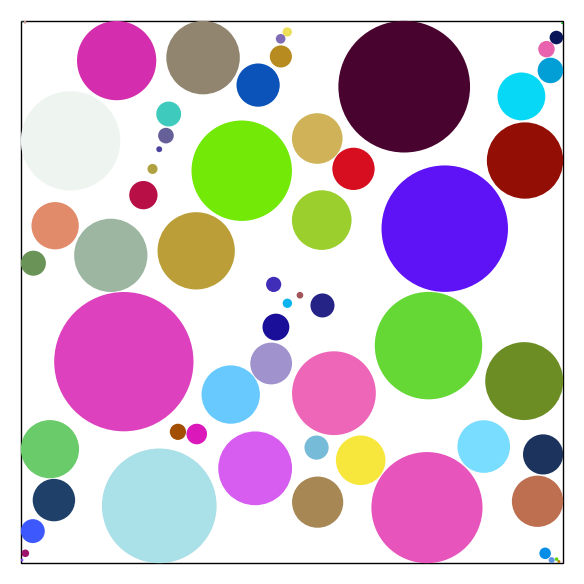
\includegraphics[width=0.3\textwidth]{square_example2.png}
    \end{center}
    \vspace{-1cm}
    \titlepage
\end{frame}

\begin{frame}
    \frametitle{The worst case for packing density?}

    %Consider circle instances with a total area of 1.

    %Conjecture: This is the worst-case instance in terms of packing density:

    \begin{center}
        \begin{tikzpicture}[scale=4]
            \squareworstcase
        \end{tikzpicture}
    \end{center}

    %Constructive proof: \emph{All} instances can be packed in this square.

\end{frame}

\begin{frame}
    \frametitle{Constructing the worst-case area}

    \begin{columns}
        \begin{column}{0.5\textwidth}
            \begin{align*}
                \Psi
                &= \left(2r + 2\frac{r}{\s}\right)^2\\
                &= r^2\left(2+\s\right)^2\\
                &= \frac{\frac 1 2}{\pi}\left(4+4\s+2\right)\\
                &= \frac{3+2\s}{\pi}\\
                &\approx 1.855\\
            \end{align*}
        \end{column}
        \begin{column}{0.5\textwidth}
            \begin{tikzpicture}[scale=3]
                \squareworstcaseconstruction
            \end{tikzpicture}
        \end{column}
    \end{columns}
\end{frame}

\begin{frame}
    \frametitle{Problem statement}

    \begin{center}
        \begin{tikzpicture}[scale=2]
            \bigquestion
        \end{tikzpicture}
    \end{center}
\end{frame}

\begin{frame}
    \frametitle{Observation: Splitting in half is easy}

    \begin{center}
        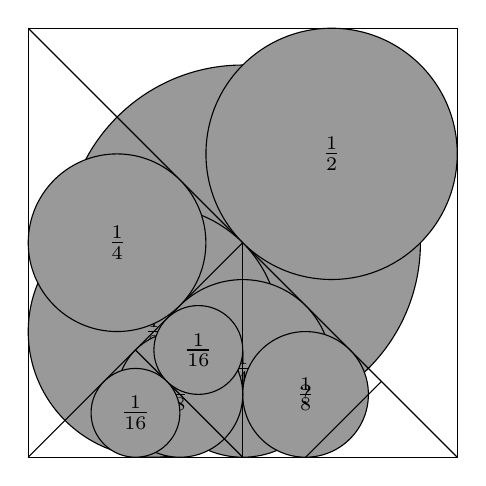
\begin{tikzpicture}[scale=4]
            \draw<+-> (0,0) rectangle (\B,\B);
            \draw<.>[filled] ({\B/2},{\B/2}) circle(0.5642) node {$1$};

            \draw<+-> (\B,0) -- (0,\B);
            \draw<.->[filled] ({\B-0.3989},{\B-0.3989}) circle(0.3989) node {$\frac 1 2$};
            \draw<.>[filled] (0.3989,0.3989) circle(0.3989) node {$\frac 1 2$};

            \draw<+-> ({\B/2}, {\B/2}) -- (0,0);
            \draw<.->[filled] (0.2820,{\B/2}) circle(0.2820) node {$\frac 1 4$};
            \draw<.>[filled] ({\B/2},0.2820) circle(0.2820) node {$\frac 1 4$};

            \draw<+-> ({\B/2}, {\B/2}) -- ({\B/2}, 0);
            \draw<.-.(1)>[filled] ({\B/2+0.1995},0.1995) circle(0.1995) node {$\frac 1 8$};
            \draw<.>[filled] ({\B/2-0.1995},0.1995) circle(0.1995) node {$\frac 1 8$};

            \draw<+-> ({\B/4}, {\B/4}) -- ({\B/2}, 0);
            \draw<.->[filled] ({\B/2-0.1410},{\B/4}) circle(0.1410) node {$\frac 1 {16}$};
            \draw<.->[filled] ({\B/4},0.1410) circle(0.1410) node {$\frac 1 {16}$};

            \draw<+-> ({\B/2+0.2}, 0) -- ({\B/4*3+0.1}, {\B/4-0.1});
            \draw<.->[filled] ({\B/2+0.1995},0.1995) node {?};
        \end{tikzpicture}
    \end{center}
\end{frame}

\begin{frame}
    \frametitle{Greedy splitting}

    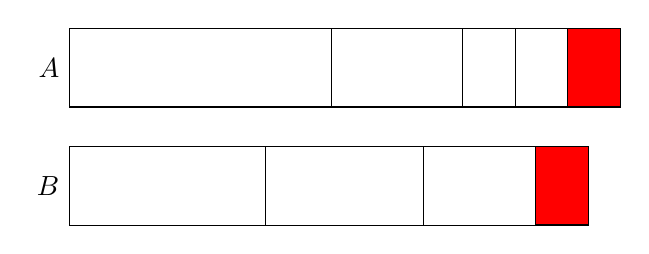
\begin{tikzpicture}[scale=10]
        \draw (0,0) -- node[left] {$A$} ++(0,0.1);
        \draw<+-> (0,-0.15) -- node[left] {$B$} ++(0,0.1);

        \draw<+-> (0,0) rectangle ++(1/3, 0.1) ++(0,-0.1) coordinate (a1);
        \draw<+-> (0,-0.15) rectangle ++(1/4, 0.1) ++(0,-0.1) coordinate (b1);
        \draw<+-> (b1) rectangle ++(1/5, 0.1) ++(0,-0.1) coordinate (b2);
        \draw<+-> (a1) rectangle ++(1/6, 0.1) ++(0,-0.1) coordinate (a2);
        \draw<+-> (b2) rectangle ++(1/7, 0.1) ++(0,-0.1) coordinate (b3);
        \draw<+-> (a2) rectangle ++(1/15, 0.1) ++(0,-0.1) coordinate (a3);
        \draw<+-> (a3) rectangle ++(1/15, 0.1) ++(0,-0.1) coordinate (a4);

        \draw<+(1)>[fill=red] (a4) rectangle ++(1/15, 0.1) ++(0,-0.1) coordinate (a5);
        \draw<+(1)>[fill=red] (b3) rectangle ++(1/15, 0.1) ++(0,-0.1) coordinate (b4);
    \end{tikzpicture}

    \vspace{1cm}

    \begin{block}<+(-2)->{Split property:}
        All elements of larger group $\ge$ groups' difference.
    \end{block}
\end{frame}

\begin{frame}
    \frametitle{Hat shape}

    \begin{center}
        \begin{tikzpicture}[scale=3]
            \hatsimple
        \end{tikzpicture}
    \end{center}
\end{frame}

%\begin{frame}
%    \frametitle{}
%
%    \begin{center}
%        \begin{tikzpicture}[scale=3]
%            \hatconstruction
%        \end{tikzpicture}
%    \end{center}
%\end{frame}

\begin{frame}
    \frametitle{Packing hats in a square}

    \begin{center}
        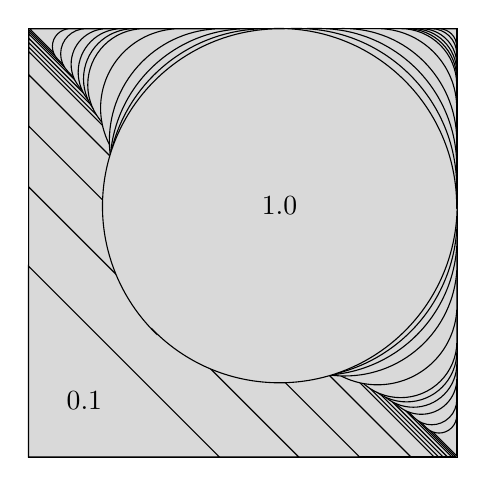
\begin{tikzpicture}[scale=4]
            \foreach \x in {0.5,0.495,0.49,0.48,0.47,0.46,0.45,0.4,0.3,0.2,0.1,0} {
                \only<+> {
                    \hatsinsquare{\x}
                }
            }
        \end{tikzpicture}
    \end{center}
\end{frame}

\begin{frame}
    \frametitle{Packing hats in a hat}

    \begin{center}
        \begin{tikzpicture}[scale=3]
            \foreach \x in {0.5,0.495,0.49,0.48,0.47,0.46,0.45,0.4,0.3,0.2,0.1,0} {
                \only<+> {
                    \hatsinhat{\x}{0}
                }
            }
        \end{tikzpicture}
    \end{center}
\end{frame}

\begin{frame}
    \frametitle{Rounding all hats does not affect the packing}

    \begin{center}
        \begin{tikzpicture}[scale=3]
            \foreach \x in {0,0.1} {
                \only<+> {
                    \hatsinhat{0.3}{\x}
                }
            }
        \end{tikzpicture}
    \end{center}
\end{frame}

\begin{frame}
    \frametitle{Example packings}

    \begin{center}
        \includegraphics<1>[width=0.5\textwidth]{square_example.png}
        \includegraphics<2>[width=0.5\textwidth]{square_example2.png}
        \includegraphics<3>[width=0.5\textwidth]{square_example3.png}
        \includegraphics<4>[width=0.5\textwidth]{square_example4.png}
    \end{center}
\end{frame}

\begin{frame}
    \frametitle{Possible extensions}

    \begin{columns}
        \begin{column}{0.5\textwidth}
            \begin{itemize}[<+->]
                \item Online?
                \item Other containers
                    \begin{itemize}
                        \item isosceles right triangles \cmark
                        \item \alert<12->{equilateral triangles}?
                        \item general triangles?
                        \item rectangles?
                        \item regular $n$-gons?
                        \item circles?
                    \end{itemize}
                \item “What about 3D?”
                    \begin{itemize}
                        \item Packing spheres into a cube?
                    \end{itemize}
            \end{itemize}
        \end{column}
        \begin{column}{\textwidth}
            \includegraphics<+->[width=0.5\textwidth]{triangle_example.png}
        \end{column}
    \end{columns}
\end{frame}

\end{document}
